% 2024 - PPGE/FURG
% - Alisson T. G. Fiorentin, alisson.fiorentin@gmail.com
% 2025 - Ago - UFC Quixadá
% - David Sena Oliveira, sena@ufc.br
% - Paulo de Tarso Guerra, paulodetarso@ufc.br

%%%%%%%%%%%%%%%%%%%%%%%% CONFIGURAÇÕES DE INICIO DO DOCUMENTO %%%%%%%%%%%%%%%%%%%%%%%

\documentclass[a4paper, 12pt, twoside]{article}
\usepackage{estilo}

\usepackage{enumitem}

\title{APLICAÇÃO DA METODOLOGIA SCRUM NO DESENVOLVIMENTO DE UM SISTEMA DE GESTÃO PARA ARENAS ESPORTIVAS}

\author{%
  Sávio de Carvalho Soares\authorinfo{saviocarvalho@alu.ufc.br} \\
  Francisco Samuel Cabral Leitão\authorinfo{fsamuel@alu.ufc.br}\\
  Leonara de Medeiros Braz\authorinfo{leonara@ufc.br} 
}
\date{}

\begin{document}
\maketitle

%%%%%%%%%%%%%%%%%%%%% RESUMO E ABSTRACT %%%%%%%%%%%%%%%%%%%%%%%%%%%%%%

\qabstract{Resumo}{Palavras-chave}{ODS}{% Mantenha esse % colado no {
A gestão de agendamentos em centros esportivos de pequeno e médio porte, como a Arena Júnior Bocão em Floriano-PI, frequentemente depende de métodos manuais como cadernos, planilhas ou aplicativos de mensagens. Tais abordagens são suscetíveis a falhas humanas, como o sobreagendamento (duplo booking), dificuldade no controle financeiro e ausência de métricas para a tomada de decisão estratégica, limitando o potencial de crescimento do negócio. Diante deste cenário, o objetivo deste trabalho é apresentar o processo de desenvolvimento do ArenaHub, um sistema web projetado para otimizar e automatizar a gestão de horários, pagamentos e comunicação em quadras esportivas. 
}{ % Palavras-chave
    Engenharia de Software. Metodologias Ágeis. Scrum. Sistema de Agendamento. Gestão Esportiva.
}{ % Objetivos ODS
    Trabalho Decente e Crescimento Econômico.
}

\qabstract{Abstract}{Keywords}{SDG}{% Mantenha esse % colado no {
The management of sports centers often relies on manual methods prone to human errors, such as double bookings, and lacks proper financial control and performance metrics. This paper presents the development process of ArenaHub, a web system designed to optimize and automate the management of sports venues. The project was conducted using the Scrum framework, organized in 15-day Sprints and in direct collaboration with a real client. The resulting system features a centralized calendar, online booking, automated payments via Pix with a reservation expiration logic, and a management dashboard with key performance indicators. This work demonstrates the viability of applying agile practices to develop high-impact technological solutions for businesses, addressing practical management challenges.
}{ % Keywords
    Software Engineering. Agile Methodologies. Scrum. Scheduling System. Sports Management.
}{ % Objetivos ODS em inglês
    Decent Work and Economic Growth.
}

%%%%%%%%%%%%%%%%%%%%%%%%%%%%%% SEÇÕES %%%%%%%%%%%%%%%%%%%%%%%%%%%%%

\section{Introdução}

A gestão de centros esportivos de pequeno e médio porte, como quadras de areia e campos society, enfrenta desafios operacionais significativos. A dependência de métodos manuais (cadernos, planilhas ou aplicativos de mensagens) é suscetível a falhas como o sobreagendamento (\textit{duplo booking}), além de dificultar o controle financeiro e a coleta de dados para decisões estratégicas. Tais limitações representam um obstáculo para a otimização da receita e o crescimento sustentável do negócio.

Diante desse cenário, este trabalho apresenta o processo de desenvolvimento do ArenaHub, um sistema web concebido para automatizar e profissionalizar a administração de arenas esportivas, centralizando o calendário de horários, o agendamento e o pagamento via Pix. O objetivo principal deste artigo é descrever a aplicação da metodologia ágil Scrum no desenvolvimento desta solução de software para um cliente real, a arena Júnior Bocão, detalhando as etapas do processo desde o levantamento de requisitos até a implementação das funcionalidades em ciclos incrementais.

A metodologia adotada para a condução do projeto foi o Scrum, um \textit{framework} ágil que permite a entrega de valor de forma contínua e adaptativa \cite{SchwaberSutherland2020}. O trabalho foi organizado em \textit{Sprints} de 15 dias, com cerimônias regulares para planejamento, sincronização e revisão. Este estudo demonstra a viabilidade de aplicar práticas formais de engenharia de software para criar soluções tecnológicas de alto impacto para pequenas empresas, resolvendo problemas práticos de gestão e gerando um produto de software escalável.

\section{Desenvolvimento}

O desenvolvimento do ArenaHub foi motivado pela necessidade de transpor os desafios operacionais e de gestão de receita identificados em centros esportivos de pequeno porte. A fase de \textbf{Discovery} foi conduzida em parceria direta com a \textbf{Arena Júnior Bocão}, que atuou como cliente real e \textit{stakeholder}, validando como desafios principais a eliminação do \textit{duplo booking} e a automação do controle financeiro. Para definir os requisitos do sistema, o processo de elicitação foi realizado por meio de entrevistas semiestruturadas, método que permitiu à equipe explorar as dores e necessidades do gestor, capturando insights práticos não mapeados previamente.

\newcommand{\originalintextsep}{\intextsep} % Guarda o valor original

% ** [Ajuste de Espaçamento para Tabela] **
\setlength{\intextsep}{5pt plus 3pt minus 3pt}

A gestão do projeto foi inteiramente estruturada com base na metodologia \textbf{Scrum} \cite{scrum-guia-projetos-ageis}. A adoção do \textit{framework} ágil foi crucial para garantir que o produto final atendesse às demandas do cliente de forma adaptativa e eficiente, sendo o trabalho organizado em \textbf{Sprints de 15 dias}. O gerenciamento do \textit{Product Backlog} e do \textit{Sprint Backlog} foi realizado através da ferramenta \textbf{ClickUp}, garantindo transparência e rastreabilidade das atividades ao longo do desenvolvimento.

A aplicação do Scrum exigiu um time multifuncional e auto-gerenciável, composto por cinco membros do corpo discente, cujos papéis estão detalhados na Tabela \ref{tab:composicao_time}. A multifuncionalidade dos Developers garantiu todas as habilidades necessárias para criar valor a cada Sprint, incluindo a criação do plano diário, a introdução de qualidade pela Definição de Pronto e a adaptação em direção à Meta da Sprint \cite{scrum-guia-projetos-ageis}. As cerimônias de sincronização e revisão foram estabelecidas com a seguinte frequência: A estrutura de papéis foi definida da forma que é apresentada na Tabela \ref{tab:composicao_time}. A multifuncionalidade do time (Developers) permitiu que os membros possuíssem todas as habilidades necessárias para criar valor a cada Sprint. As responsabilidades dos Developers incluíram a criação do plano diário na Daily Scrum, a introdução de qualidade pela Definição de Pronto e a adaptação do plano em direção à Meta da Sprint \cite{scrum-guia-projetos-ageis}. As cerimônias de sincronização e revisão foram estabelecidas com a seguinte frequência:

\begin{itemize}[noitemsep, nolistsep]
 \item \textbf{Daily Scrum (Reuniões Diárias):} Realizadas pontualmente às \textbf{19:30} (de segunda a sexta-feira) para garantir o alinhamento técnico da equipe, discutir o progresso diário e remover impedimentos.
 \item \textbf{Sprint Planning, Retrospective e Review:} Conduzidas em conjunto no dia seguinte ao término de cada \textit{Sprint} (geralmente às 19:30). O ciclo integrado permitiu uma rápida adaptação e o planejamento imediato do próximo ciclo de desenvolvimento.
 \item \textbf{Mentoria e Revisão (Professora Braz):} A \textbf{Sprint Review} contou com a participação periódica da Professora Leonara Braz (UFC Quixadá), que forneceu orientação estratégica e técnica, sendo fundamental para o sucesso e o rigor acadêmico do projeto.
\end{itemize}

\begin{table}[htb]
    \caption{Composição e Responsabilidades do Time Scrum}
    \label{tab:composicao_time}
    \centering
    \footnotesize
    \begin{tabular}{|p{3cm}|p{3.5cm}|p{7cm}|}
        \toprule
        \textbf{Membro (Nome Fictício)} & \textbf{Papel no Scrum} & \textbf{Foco Principal e Responsabilidades} \\
        \midrule
        \textbf{Sávio Soares} & Scrum Master & Responsável por estabelecer o Scrum e treinar o time em autogerenciamento. Liderou as cerimônias diárias e atuou na remoção de impedimentos. \\
        \hline
        \textbf{Rian Lima} & Developer Back-end / Arquiteto & Responsável pelo desenvolvimento da lógica de negócio, persistência (JPA/PostgreSQL) e integrações críticas (PIX/Asaas). \\
        \hline
        \textbf{Samuel Leitão} & Developer Front-end / UX & Focado na experiência do usuário e na implementação da interface (Next.js/React). Garantiu o incremento inspecionável. \\
        \hline
        \textbf{Renan Soares} & Developer Back-end / Analista de Requisitos & Atuou na tradução das necessidades do cliente (Arena Júnior Bocão) em itens claros do Product Backlog e no desenvolvimento de \textit{features} críticas. \\
        \midrule
        \textbf{Douglas Eduardo} & Developer Front-end & Focado na implementação da interface (Next.js/React). Garantiu o incremento inspecionável. \\
        \bottomrule
    \end{tabular}
\end{table}

O compromisso com a qualidade do software foi reforçado pela adoção das práticas de \textbf{TDD (Test-Driven Development)} e \textbf{BDD (Behavior-Driven Development)}, sob a orientação da Professora Paulyne Jucá (UFC Quixadá).

\begin{figure}[!htb]
\caption{Exemplo de Requisito de Geração de PIX para Agendamento Fixo formatado em BDD no ClickUp.}
\label{fig:bdd_card}
\centering
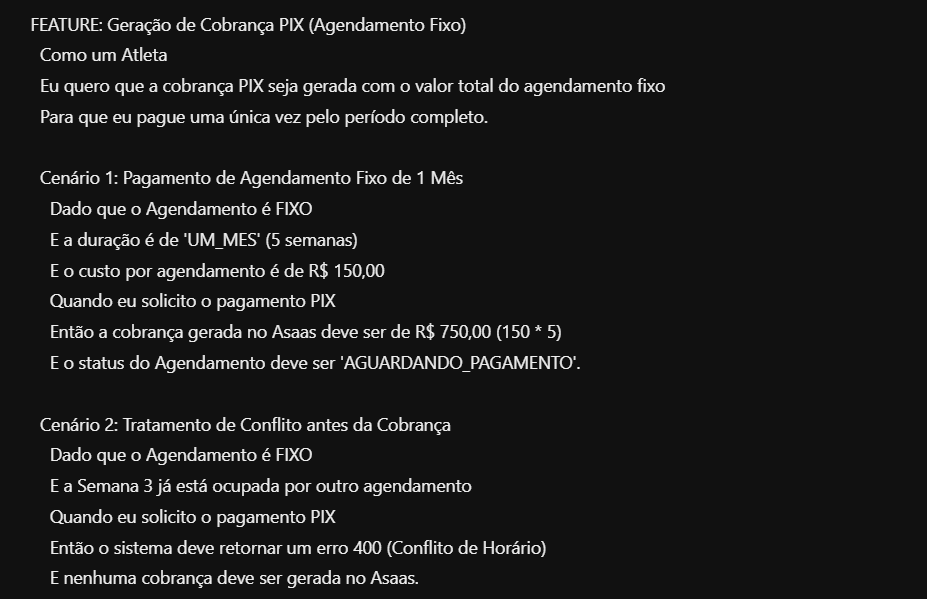
\includegraphics[width=1.0\textwidth]{figs/BDD_Pagamento_PIX_AG_FIXO.png}
{\footnotesize Fonte: Elaborado pelos autores}
\end{figure}

\subsection{Produto desenvolvido}

O principal requisito funcional, a \textbf{Busca e Reserva Online}, permite que os usuários visualizem a disponibilidade de todas as quadras em tempo real e realizem o agendamento de forma autônoma, eliminando a dependência de métodos manuais e a possibilidade de erros.

Para garantir a eficiência financeira, o sistema conta com a \textbf{Automação de Pagamentos via Pix}. Uma vez que o atleta escolhe um horário, uma reserva provisória é criada e cancelada automaticamente caso o pagamento não seja confirmado em até 10 minutos. Essa lógica de expiração assegura que os horários não fiquem bloqueados indevidamente, otimizando a taxa de ocupação e a receita da arena.
\vspace{0.2cm}

Pensando no engajamento da comunidade de atletas, foram desenvolvidas \textit{features} sociais. A funcionalidade de \textbf{Jogos Abertos} permite que jogadores encontrem partidas com vagas disponíveis, facilitando a organização de "rachas". Complementando essa função, o \textbf{Sorteador de Times} oferece uma ferramenta simples para dividir os jogadores de forma justa.

Para a melhoria contínua dos serviços, o sistema inclui um \textbf{Módulo de Avaliações}, onde os atletas podem fornecer feedback sobre a infraestrutura e o atendimento. Todas as interações, como agendamentos e pagamentos, geram \textbf{Notificações em Tempo Real}, mantendo todos informados.

Finalmente, para o gestor da arena, o \textbf{Painel de Gestão} centraliza todas as operações. Ele oferece uma visão completa dos indicadores de desempenho, como taxa de ocupação e faturamento, e permite o gerenciamento completo das quadras, incluindo a configuração de preços e horários.

\begin{figure}[!htb]
\caption{Busca de horários de uma Arena}
\label{fig:backlog_clickup}
\centering
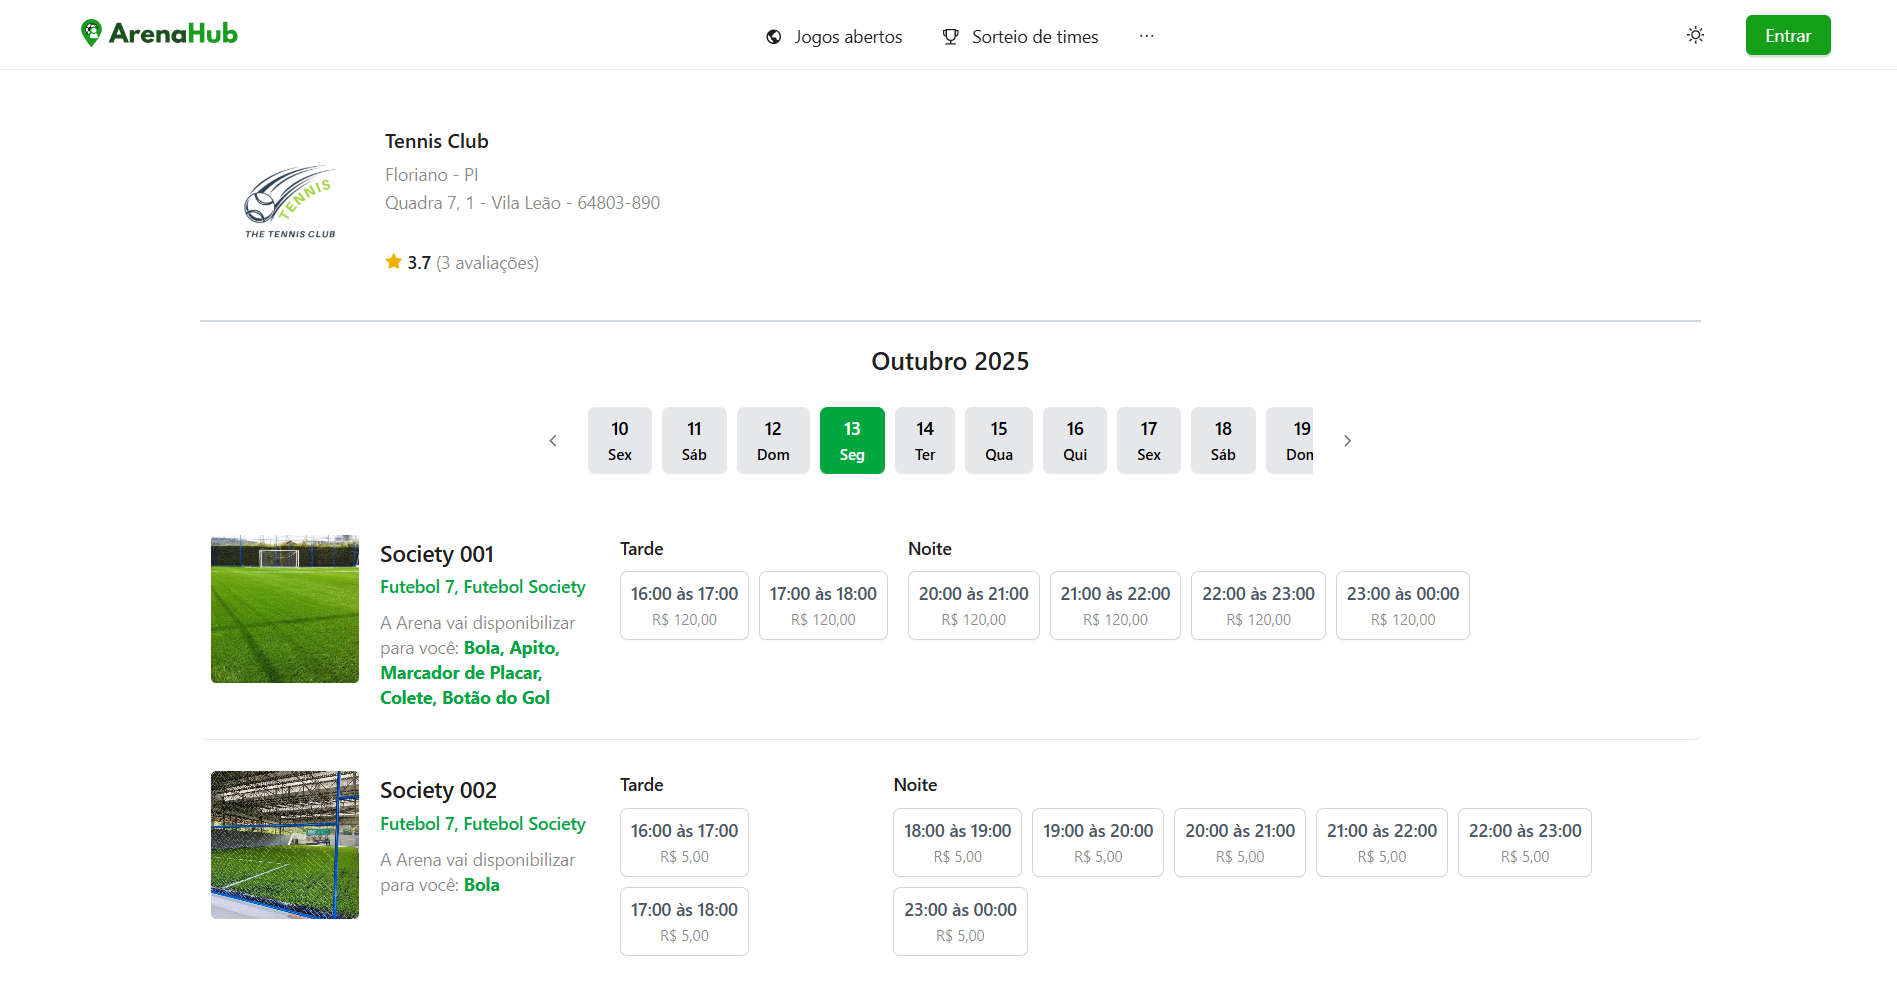
\includegraphics[width=0.8\textwidth]{figs/print_horarios_livres.png}\\
{\footnotesize Fonte: Elaborado pelos autores}
\end{figure}


\section{Considerações Finais}

Este artigo descreveu a aplicação bem-sucedida da metodologia Scrum no desenvolvimento do ArenaHub para um cliente real. A utilização do framework ágil foi fundamental para a organização, o aprendizado prático da equipe e a entrega contínua de um produto de software de qualidade. A colaboração contínua com a arena parceira, estruturada pelos eventos do Scrum, confirmou a eficácia do método para projetos acadêmicos com interação externa, servindo como uma ponte valiosa entre o conhecimento formal de engenharia de software e os desafios do mercado.

O ArenaHub, como produto final, responde diretamente aos problemas operacionais levantados, mitigando o \textit{duplo booking} pela centralização do calendário, otimizando o controle financeiro com a automação via Pix e oferecendo métricas para a tomada de decisão estratégica. Como próximos passos, reconhecemos a necessidade de validação e refinamento da solução. Pretendemos realizar testes de usabilidade e avaliar a experiência com o cliente real, garantindo a melhoria contínua do sistema.
%%%%%%%%%%%%%%%%%%%%%%%%%% REFERÊNCIAS %%%%%%%%%%%%%%%%%%%%%%%%%%%%%%%%

% habilite a geração da bibliografia apenas na versão final,
% para economizar tempo de compilação no overleaf
\printbibliography

\qcentersection{AGRADECIMENTOS}

Os membros da equipe agradece principalmente à Leonara Brás por todo o empenho, coordenação e por acreditar na idéia do projeto desde o começo. Posteriormente, vai nossos agradecimentos ao resto da equipe que participaram do desenvolvimento mas não quiseram fazer parte desse trabalho, são eles: Renan Alencar, Rian Lima e Douglas Eduardo. 

\end{document}